\chapter{Experiments}

At this point of the thesis the reader should be already familiar with the notions we have introduced: the problem of finding the optimal ID set (with respect to some \textit{weight}), that it is directly related to the NP-complete problem of finding the maximal weighted independent set, that this can be solved using the MIP approach, and that we can try to do better than just let the solver work: by employing various heuristics.

Now it is the time to move our ideas into reality and test their feasibility. But before we start talking about the experiments themselves, we should try to formulate our aim, what we will be trying to establish.\\

First of all, we would like to get an idea of how the whole system and its components behave. We would like to see the changes introduced by modifying some of the key parameters, while keeping the others fixed. Even though we shan't hope for them to be orthogonal, we might at least isolate some of the parameters that are less important to the overall behavior. Preferably, in the end we should have at least some intuition into what will happen if we try X Y Z, before trying it.

Second, as we will be introducing a few broad classes of XML data to run ID set search on, we would like to find out which types are best handled by which configurations and settings. This will allow us to pick the right heuristic once we see new data.

Also, we will try to evaluate the system performance in terms of the speed of finding good heuristic results. We will try to find tweaks to make the whole process as fast as reasonably possible.

And in the end, we should be able to formulate some kind of general recommendation in form ``if you see this kind of data, do that".\\

This chapter will be structured in the following way: first we will discuss the experimental data we used, then the methodology used in conducting the experiments, followed by the actual list of experiments with their full description and results, and in the end we shall draw some final conclusions.

\section{Experimental Data}

Let us now talk about the XML data we will be using to conduct out experiments. We are using XML documents of three categories:

\begin{itemize}
	\item Realistic
	\item Realistic with artificial (converted) attributes
	\item Artificial
\end{itemize}

A short reasoning for this choice: realistic - of course, we want to see the performance in cases taken from the real world. The problem with realistic data is that sometimes, interesting values (that might or might not contain IDs) are stored as text nodes % TODO is this name consistent with what I've been defining?
instead of attributes. We might try to look at such data, convert some of these ``suspicious" values to attributes (e.g. using a smart XSL transformation), let our heuristics find the ID sets, and then translate them back to XML keys (see \ref{realistic-converted} for details).
And finally, we create completely artificial data to create inputs that will really put our heuristics to the test. This is because the realistic data often prove to be quite easy to solve - the list of candidate AMs is usually too short to be hard to solved to optimality.\\

To understand these data sets, we will talk a little about their origin and \textit{graph representation}. As mentioned earlier, % TODO link
the problem of finding the optimal ID set is in fact the problem of finding the maximum weighted independent set on a graph. Therefore, it might be interesting to actually see the graphs of these data sets and have some kind of numbers associated with them.

The former will be achieved with the help of GraphViz tool, % TODO link
where we will draw the graphs so that all the vertices represent the \textit{candidate AMs}, and the edges represent pairs of AMs that have nonempty intersection of their images (and thus cannot be in the same ID set together). Thus solving the maximal weighted IS on these graphs will be equivalent to solving our problem of optimal ID set.

The latter will come in form of tables containing information regarding the data sets, such their size, known optimum % TODO footnote explaining that we got the optimum by running GLPK w/o time limit
for $\alpha = \beta = 1$ and the numbers of vertices and edges in aforementioned graphs.

\subsection{Realistic data}

From 3 different sources we collected 6 different data sets, called \dataset{OVA1} - \dataset{OVA3}, \dataset{XMA-c}, \dataset{XMA-p} and \dataset{XMD}. Their summary is the Table \ref{table-experiments-data-realistic}, their graphs can be seen in Figure \ref{image-experiments-data-realistic}. Because the legal status of disclosing these data sets is unclear, we will refrain from identifying them beyond these artificial identifiers. Neither will they be included on the DVD distributed with this thesis.

TODO their DTD/XSD - do we have ID attributes?

TODO verify they satisfy their schemas. Converted too.

\begin{table}
  \caption{List of realistic test data files}
  \bigskip
  \label{table-experiments-data-realistic}
  \centering
  \begin{tabular}{l | r | c | c | l}
  	Name  & Size [kb] & $|V|$ & $|E|$ & Optimum \\
  	\hline
  	\dataset{OVA1}  & 4.5      & 29 & 43 & 0.45588235294117635 \\
  	\dataset{OVA2}  & 11.9     & 23 & 36 & 0.1634615384615385  \\
  	\dataset{OVA3}  & 237.6    & 31 & 47 & 0.25537156151635415 \\
  	\dataset{XMA-c} & 1 807.7  & 1  & 0  & 0.7546666666666667  \\
  	\dataset{XMA-p} & 13 748.3 & 1  & 0  & 0.2019306150568969  \\
  	\dataset{XMD}   & 1 743.0  & 17 & 15 & 0.09786094165493507 \\
  \end{tabular}
\end{table}

\begin{figure}
  \caption{Realistic data}
  \label{image-experiments-data-realistic}
  \centering
    \subfigure[\dataset{OVA1}]{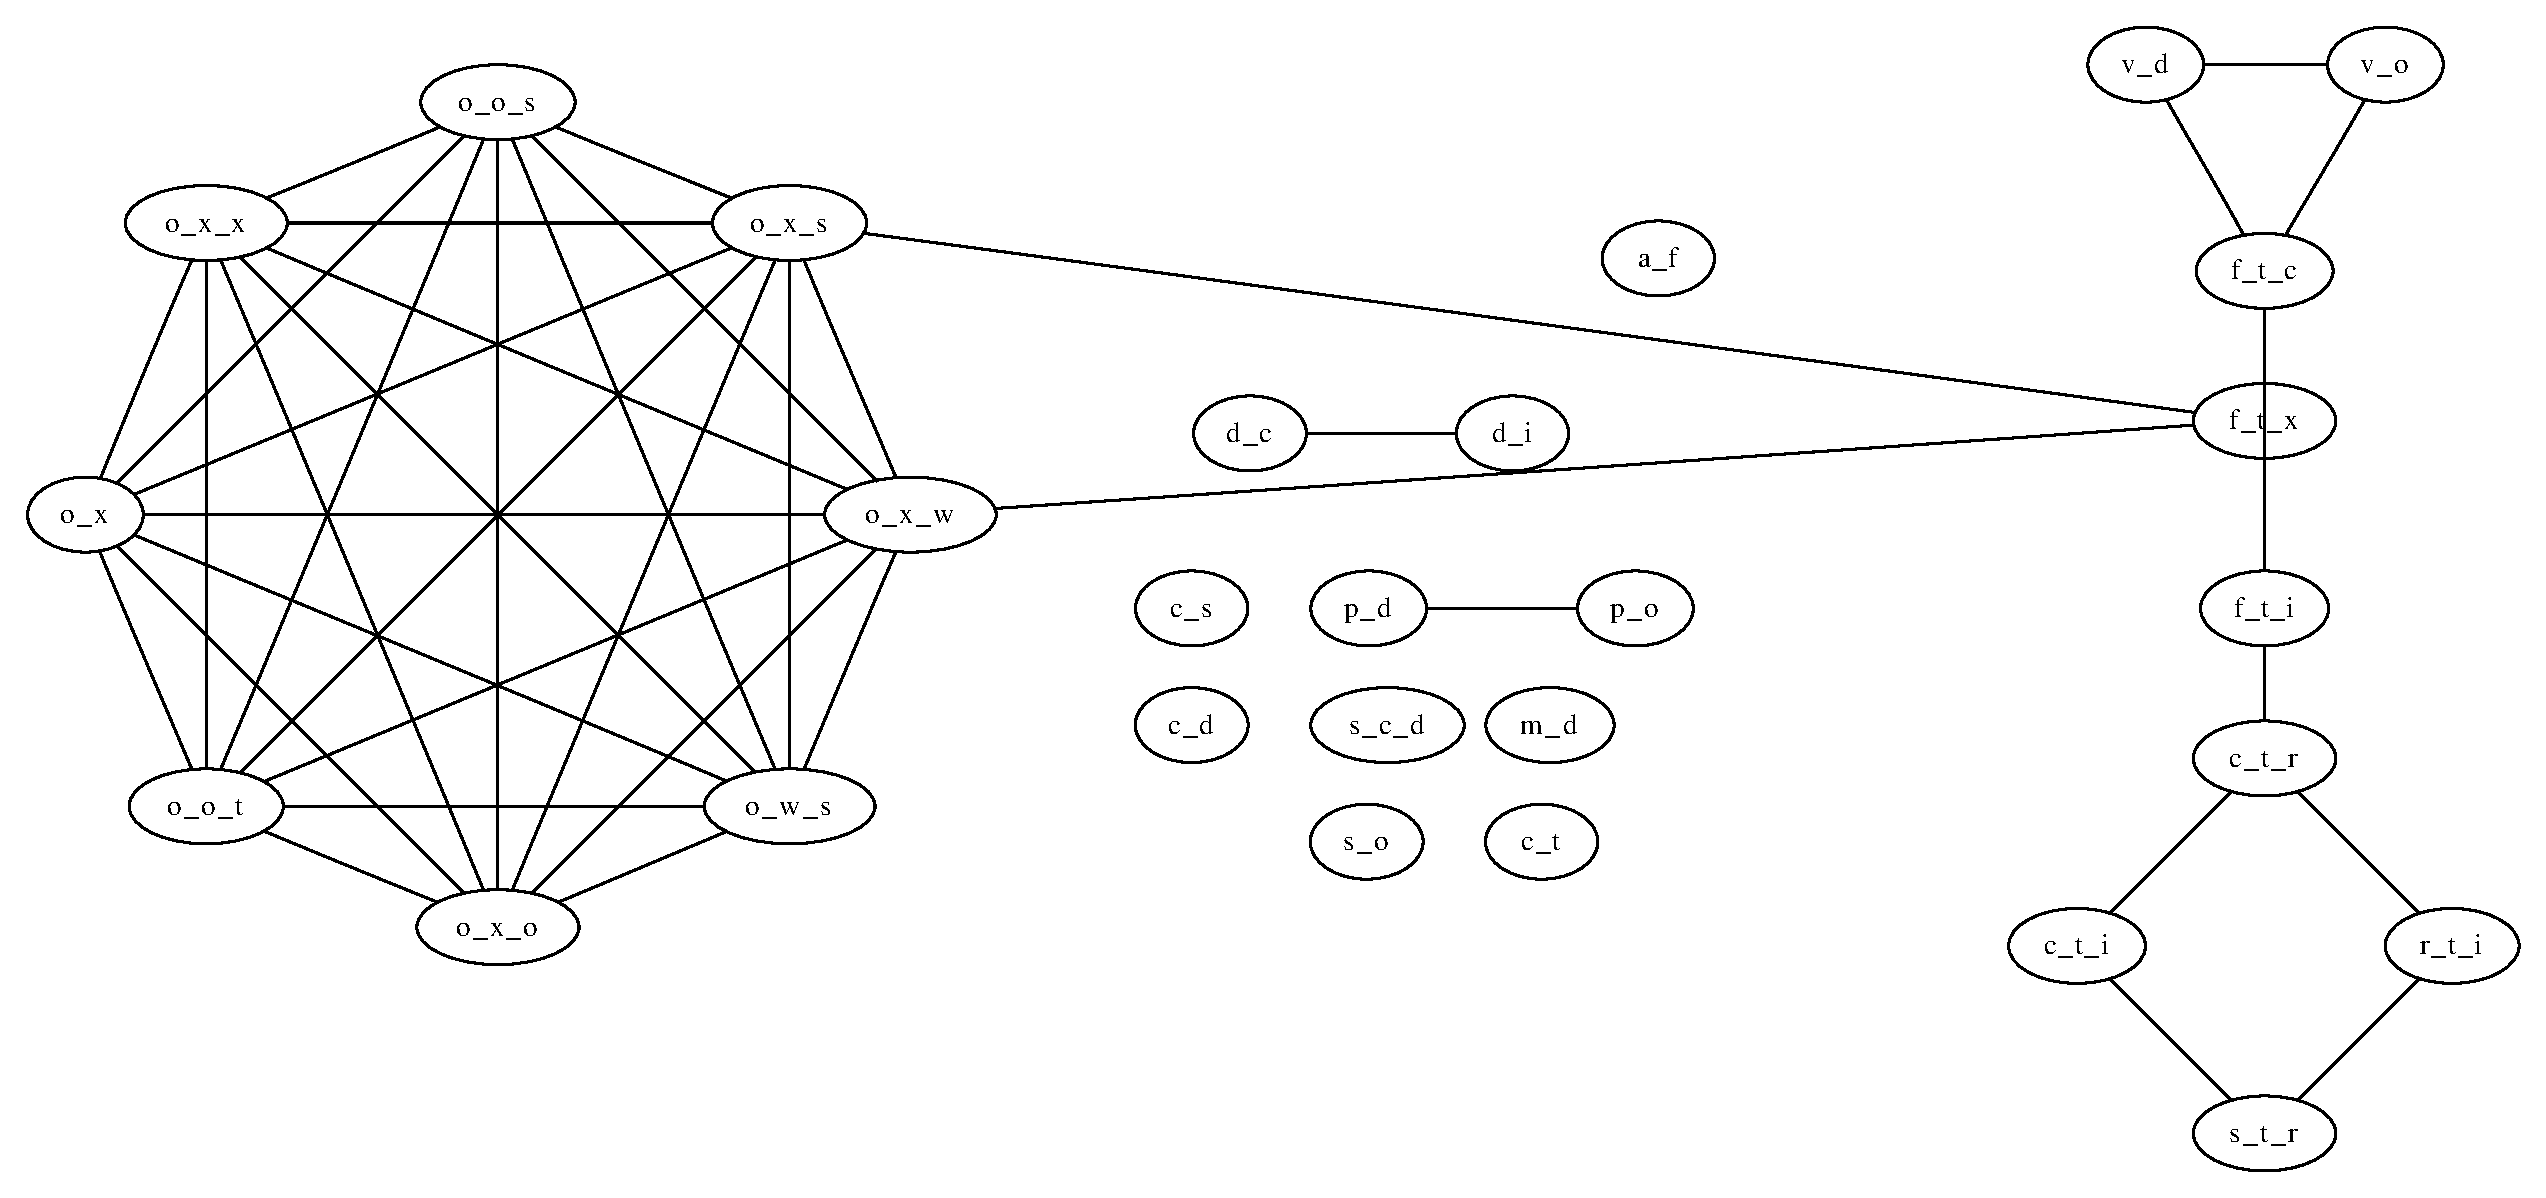
\includegraphics[width=0.45\textwidth]{images/experiments/data/realistic/OVA1}}
    \subfigure[\dataset{OVA2}]{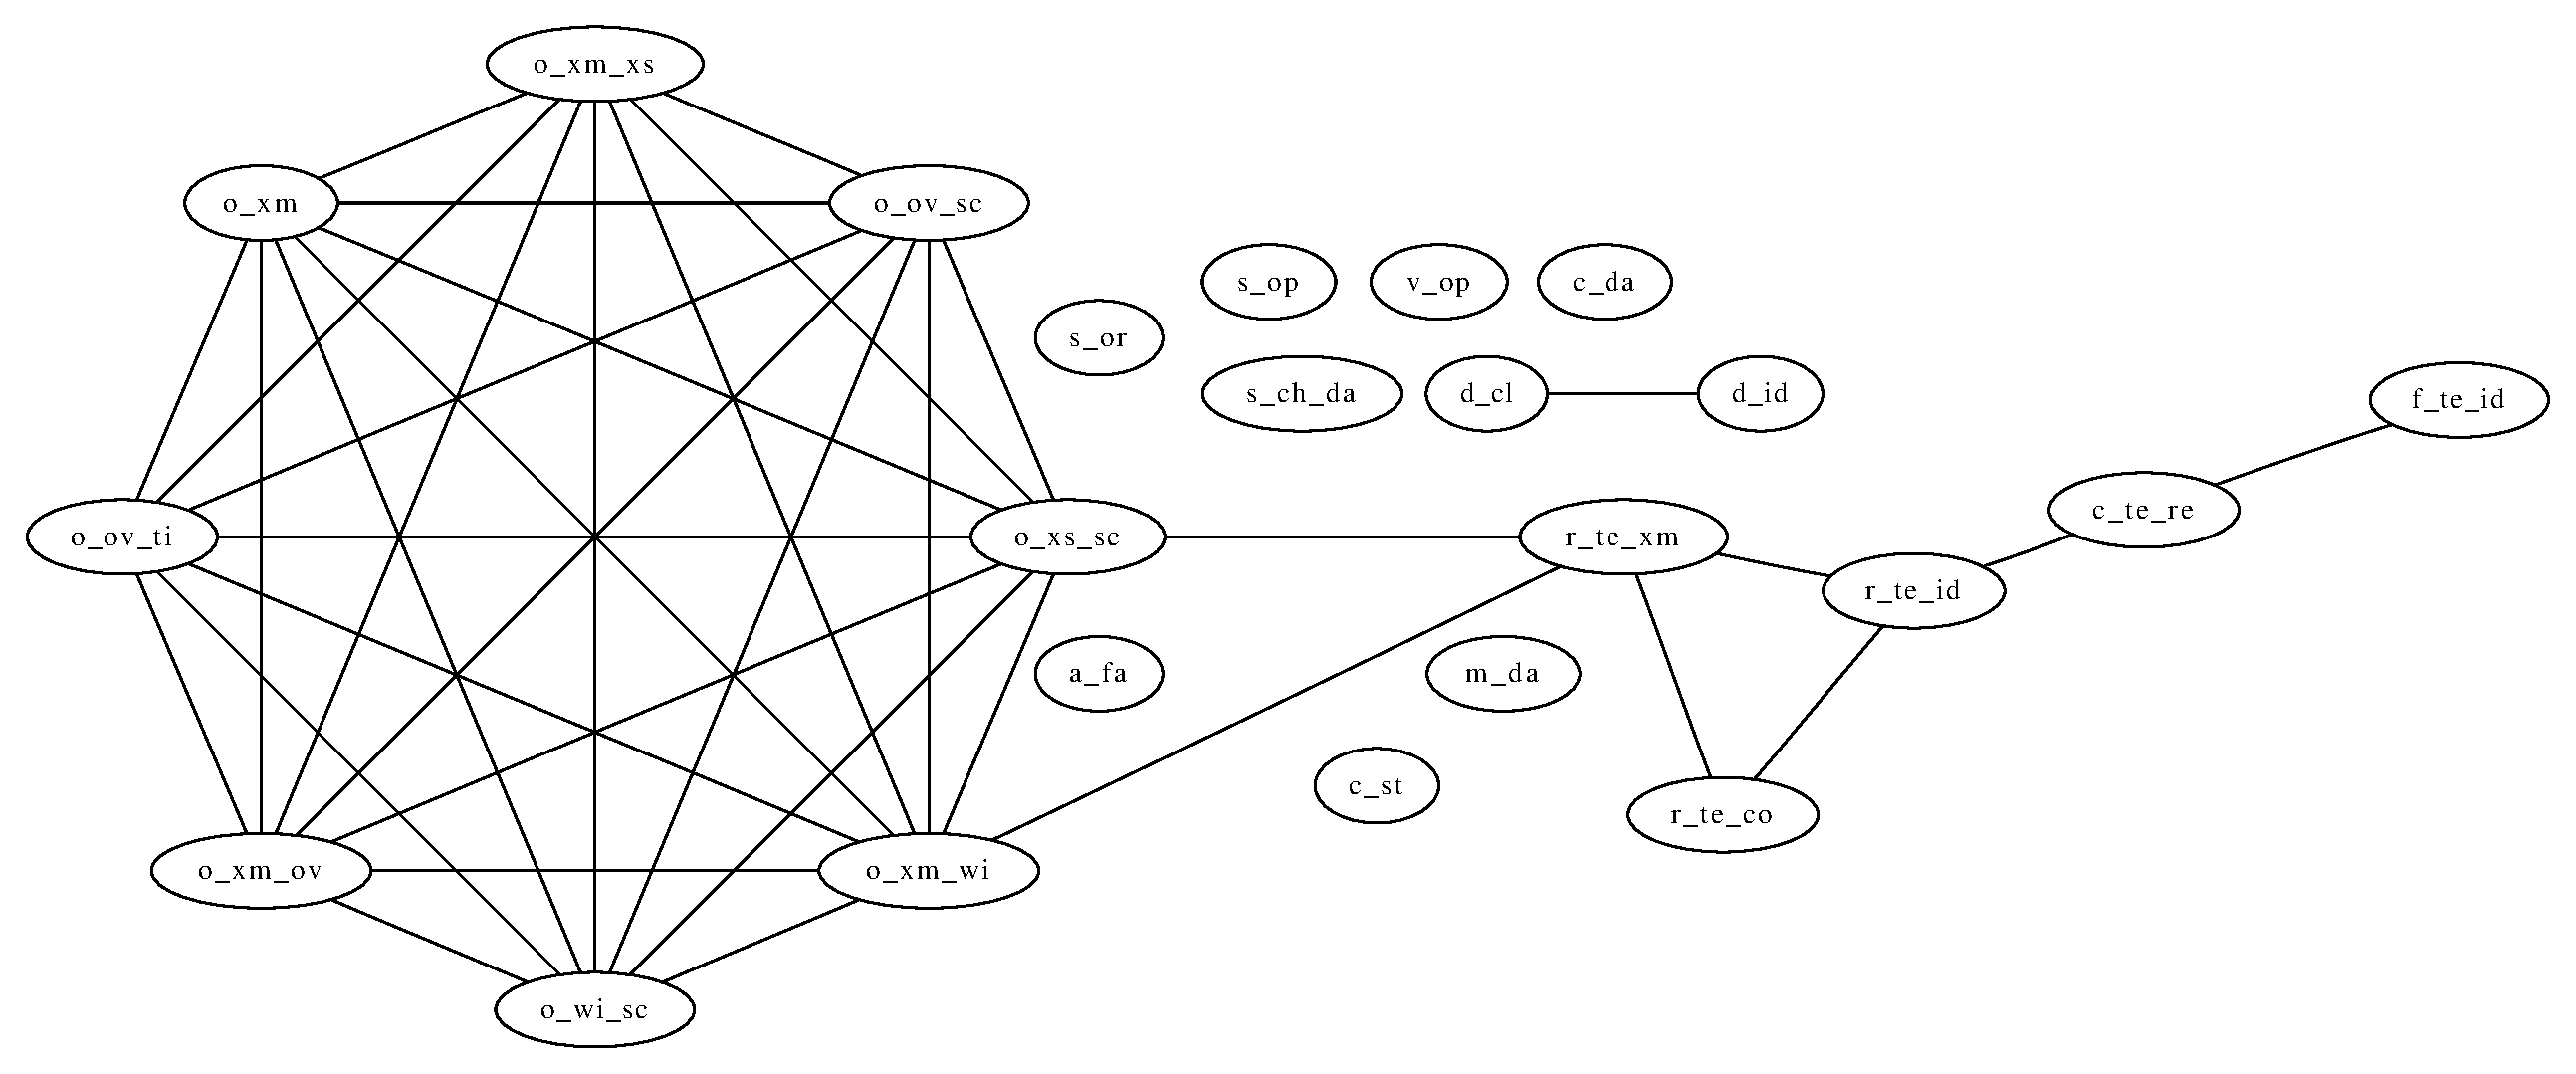
\includegraphics[width=0.45\textwidth]{images/experiments/data/realistic/OVA2}}
    \subfigure[\dataset{OVA3}]{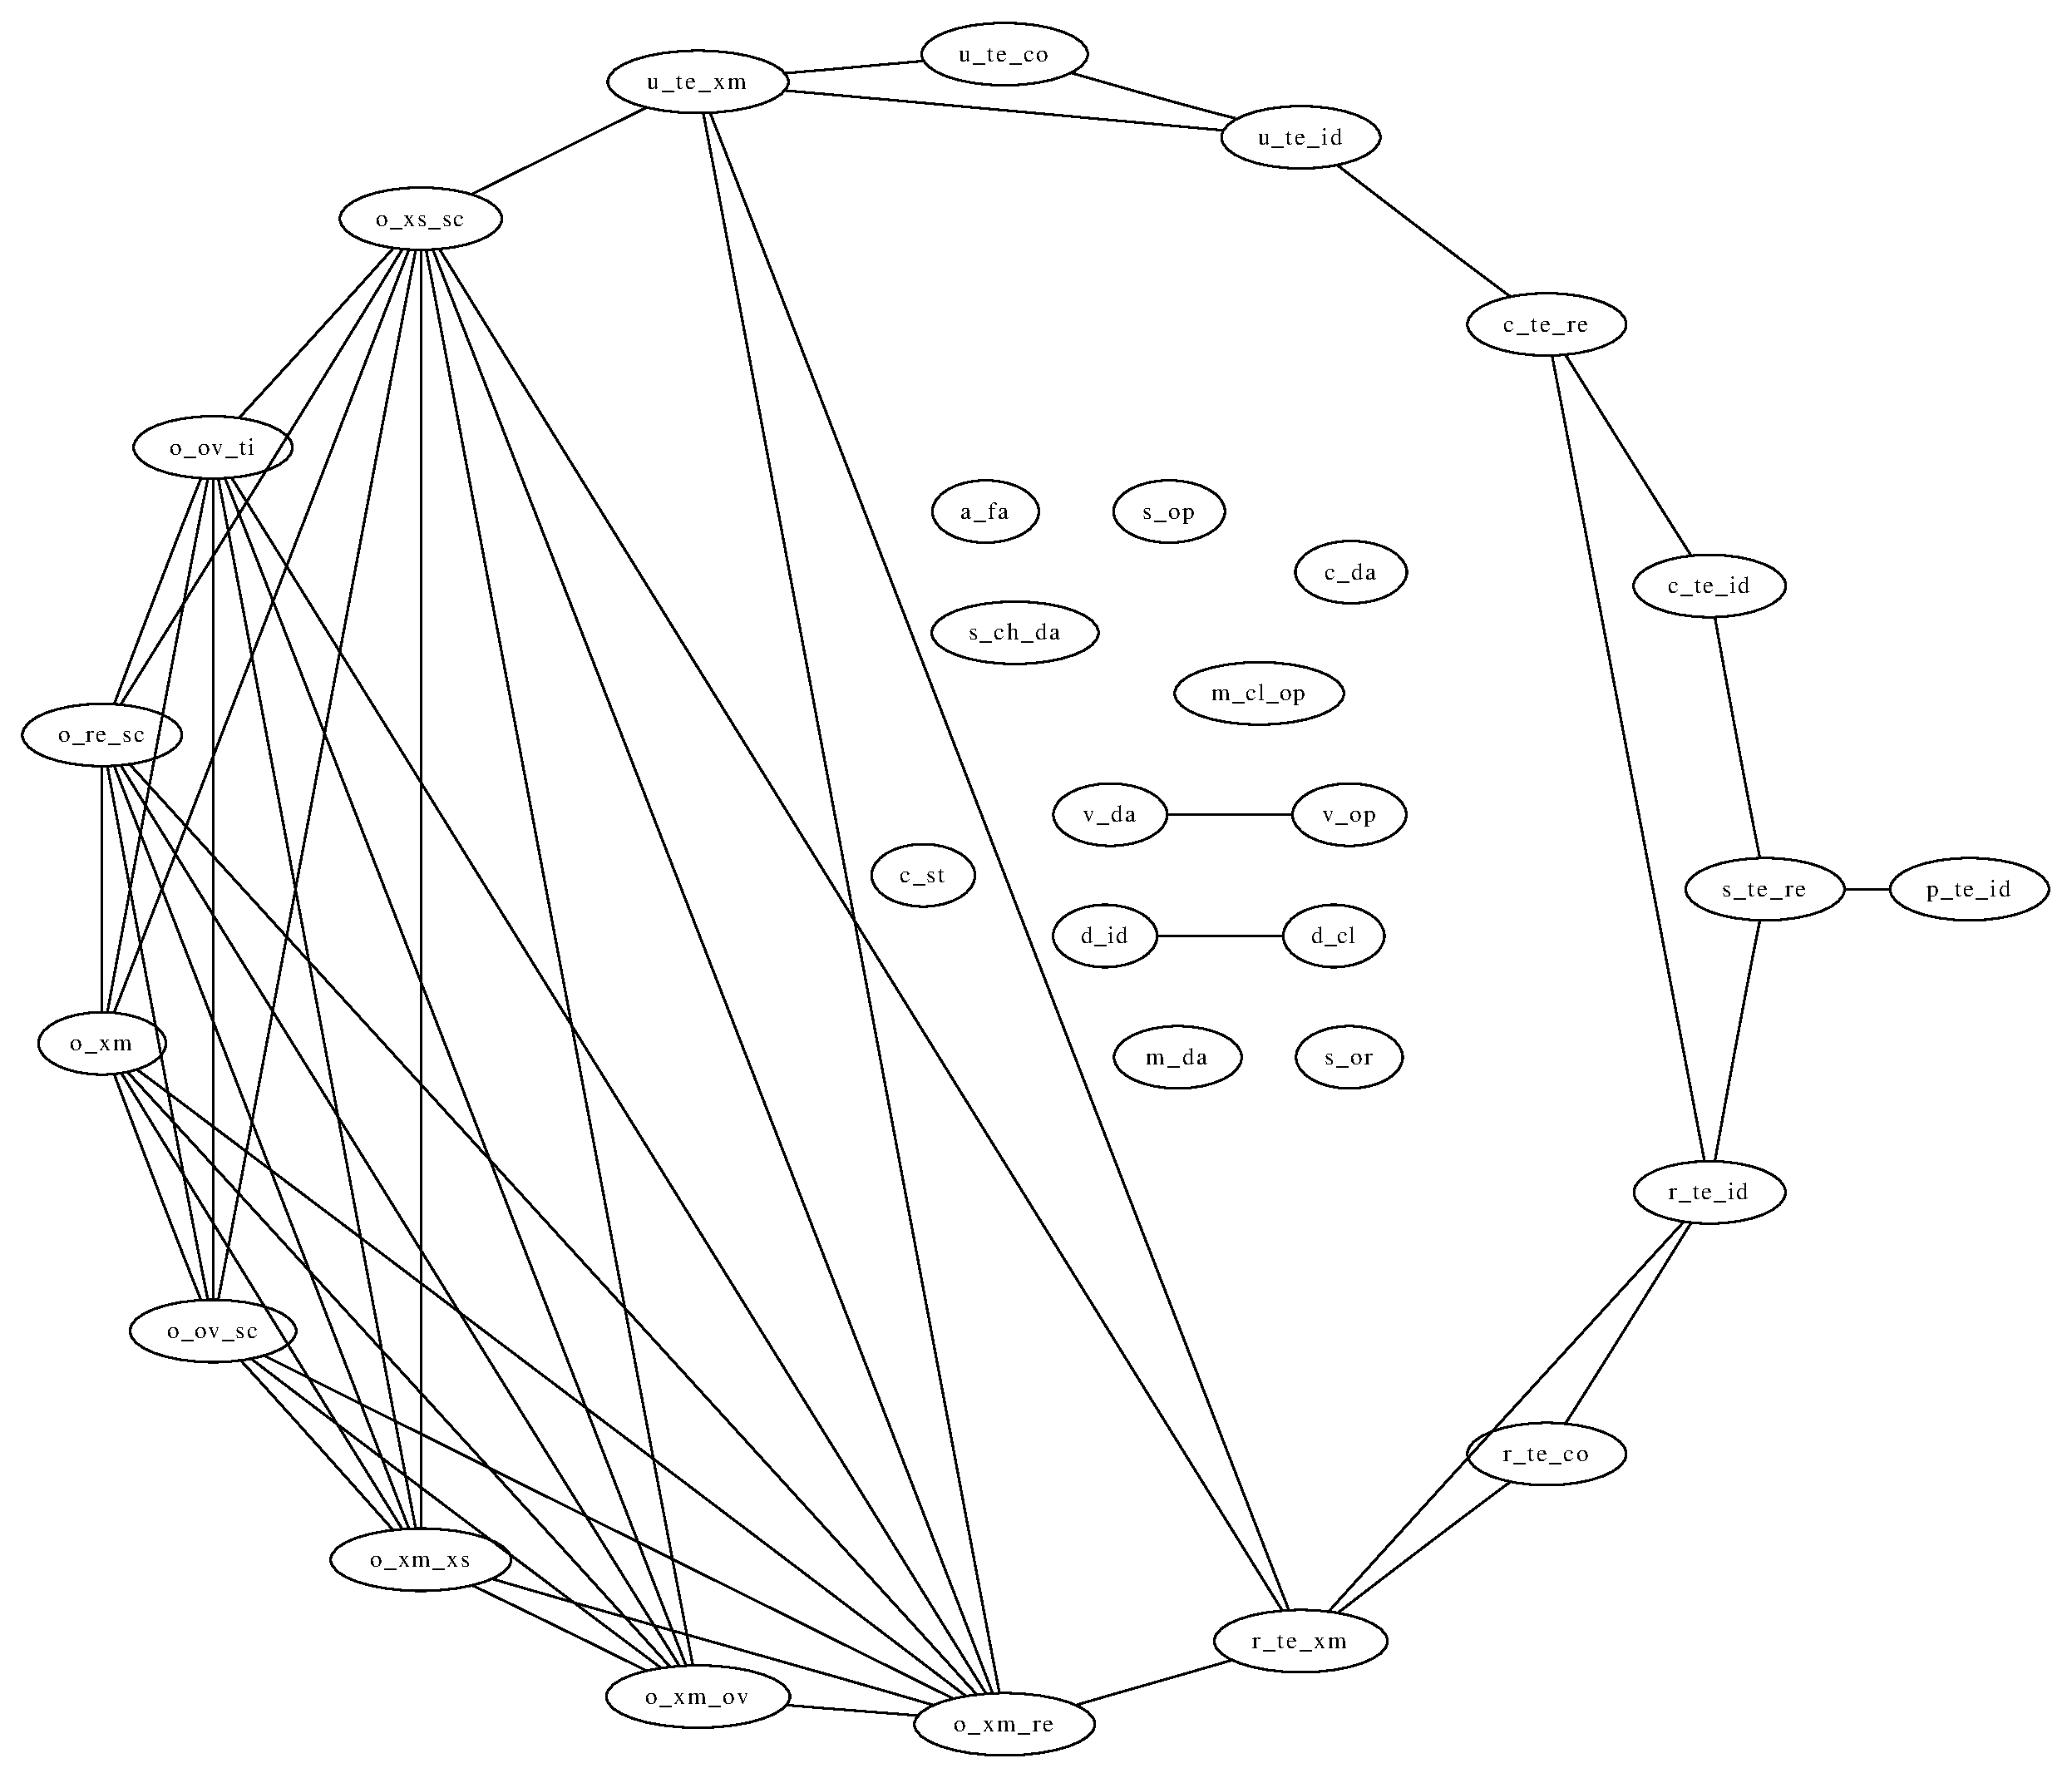
\includegraphics[width=0.45\textwidth]{images/experiments/data/realistic/OVA3}}
    \subfigure[\dataset{XMA-c}]{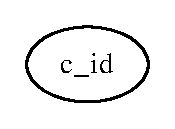
\includegraphics[width=0.08\textwidth]{images/experiments/data/realistic/XMA-c}}
    \subfigure[\dataset{XMA-p}]{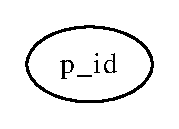
\includegraphics[width=0.08\textwidth]{images/experiments/data/realistic/XMA-p}}
    \subfigure[\dataset{XMD}]{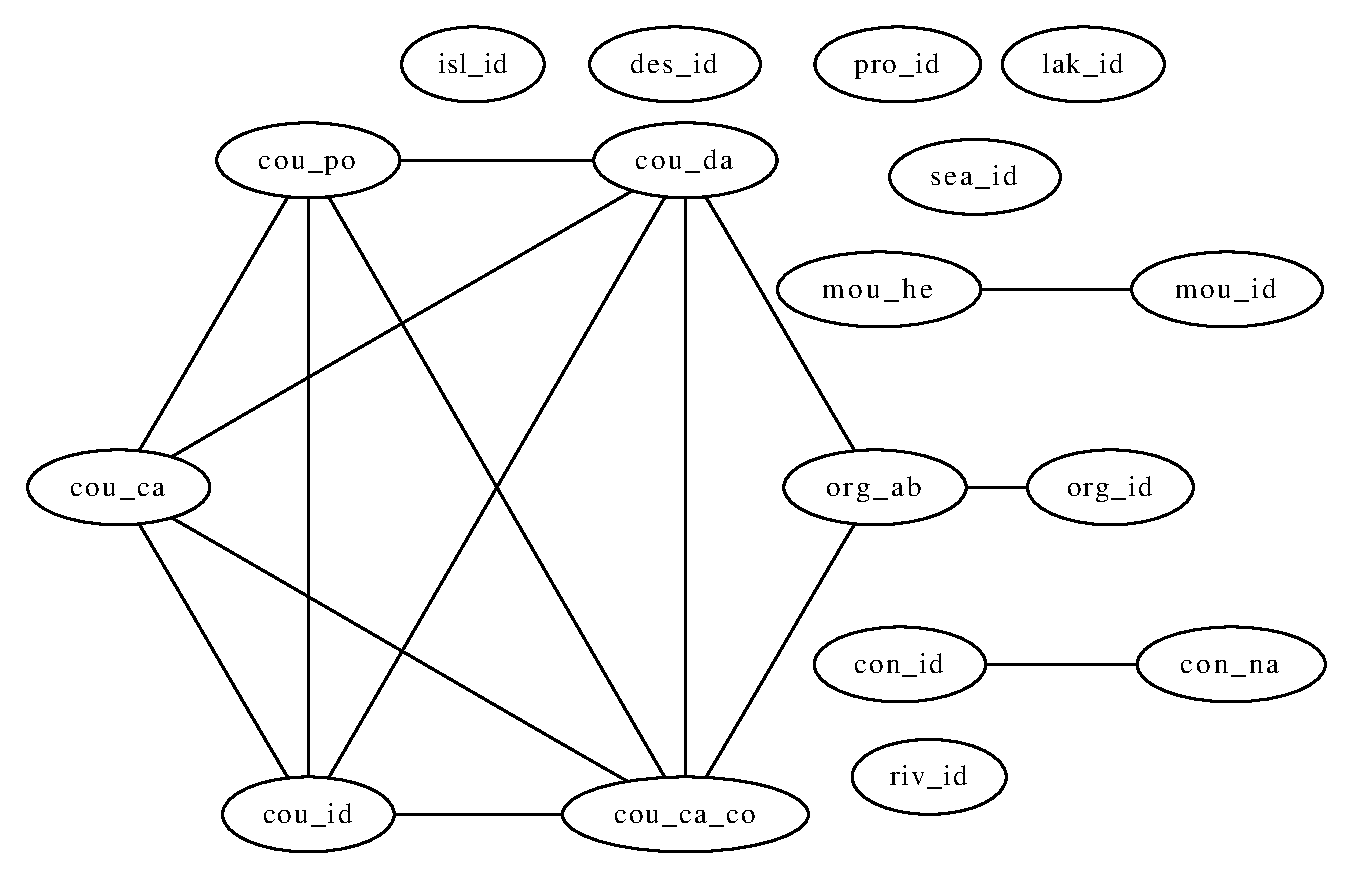
\includegraphics[width=0.45\textwidth]{images/experiments/data/realistic/XMD}}
\end{figure}

To interpret the data a little: \dataset{OVA*} sets have quite interesting and perhaps a bit challenging graphs, but are not too big. We can consider them to be the ``typical" representants.

On the other hand, the \dataset{XMA-*} sets are quite huge, but trivial: their only candidate AM will just get picked and that will be the end of the heuristic. We will see the performance of the other components of the whole system, dealing with huge data that are rather simple in the end.

Finally, the \dataset{XMD} set is quite big and at the same time has non-trivial graph representation. We should see a performance more balanced between processing and finding the ID set here.

\subsection{Realistic data with artificial attributes}
\label{realistic-converted}

We found 2 data sets to convert, \dataset{MSH} and \dataset{NTH}. Unfortunately, the same problem with disclosure as in the previous case applies here. None of these sets had any attributes before the conversion. Their summary is the Table \ref{table-experiments-data-converted}, their graphs can be seen in Figure \ref{image-experiments-data-converted}.

TODO schemas?

To address the conversion: in the case of \dataset{MSH} we found 2 elements with values looking suspiciously like a key of the records contained in the file, and converted them to be attributes of these records using a simple XSL transformation. In the case of \dataset{NTH} we converted all the values in sub-elements of the record elements to be the attributes of the records.

Why is this useful at all? Recall TODO link, where we said that ID attributes are a special case of XML keys. We can use this approach then to find XML keys: convert some suspicious data into attributes, find the optimal ID set and then create XML key based on this ID set.

\begin{table}
  \caption{List of realistic test data files with converted attributes}
  \bigskip
  \label{table-experiments-data-converted}
  \centering
  \begin{tabular}{l | r | c | c | l}
  	Name  & Size [kb] & $|V|$ & $|E|$ & Optimum \\
  	\hline
  	\dataset{MSH}  & 3 100.5 & 1 & 0 & 0.5416472778036296 \\
  	\dataset{NTH}  & 2 523.5 & 5 & 7 & 0.057918595422124436 \\
  \end{tabular}
\end{table}

\begin{figure}
  \caption{Realistic data with converted attributes}
  \label{image-experiments-data-converted}
  \centering
    \subfigure[\dataset{MSH}]{
\includegraphics[width=0.08\textwidth]{images/experiments/data/converted/MSH}}
    \subfigure[\dataset{NTH}]{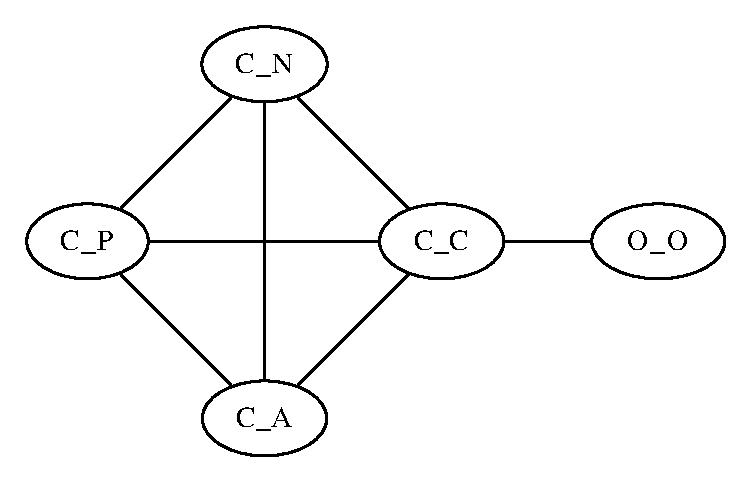
\includegraphics[width=0.45\textwidth]{images/experiments/data/converted/NTH}}
\end{figure}

Again to do a little interpretation: in the case of \dataset{MSH} we created 2 attributes, of which only one constituted a candidate AM. This is then the case similar to \dataset{XMA-*} sets: quite large data, yet only one trivial ID attribute to be found.

In the case of \dataset{NTH} we introduced more attributes, 8 to be precise. Out of them 5 proved to be candidate AMs, with 7 edges constraining them. This means we have quite a big set with relatively simple work to be done by the heuristics. This is about the change.

\subsection{Artificial data}

As soon as we started experimenting with the data coming from the real world, it was obvious that they present no real challenge to our heuristics. After we build the model, we get the most complex graphs of some 31 vertices and 47 edges (see Table \ref{table-experiments-data-realistic}). We needed to create data that would really put pressure on our heuristics, put them to a real test. Our solutions is to approach from the other side: in the end, we will be solving the equivalent of IS problem on a graph created from XML data. Why not create the XML data to contain a more complex graph in the first place? What if we could specify how many vertices and edges we want, and get the according XML?

This is actually simple. Consider the following excerpt from an XML file:

\begin{scriptsize}
\begin{verbatim}
<graph>
  <vertex0 attr="-2968876296119015800"/>
  <vertex1 attr="1729745997570096518"/>
  <vertex2 attr="-9020549659620928934"/>
  ...
  <vertex99 attr="-7545982394508643394"/>

  <vertex82 attr="0"/><vertex21 attr="0"/>
  <vertex64 attr="1"/><vertex21 attr="1"/>
  <vertex44 attr="2"/><vertex2 attr="2"/>
  ...
  <vertex96 attr="99"/><vertex40 attr="99"/>
</graph>
\end{verbatim}
\end{scriptsize}

We want to create a graph with around $v$ vertices and $e$ edges. First, we introduce $v$ elements with names \texttt{vertex0} - \texttt{vertex\{V-1\}}. To constitute an AM, they need an attribute \texttt{attr}, but with large enough random values, so that these values won't conflict with any others. Second, for each of the $e$ edges we pick two \texttt{vertex*} elements at random, and give them the same value of their \texttt{attr}. This will ensure they cannot share the same ID set, thus effectively creating the edge in the graph representation.

The pseudocode for this is in Listing \ref{listing-random-data}.

\begin{algorithm}
\caption{Random XML data creation}
\label{listing-random-data}
\begin{algorithmic}
\REQUIRE $v$ requested number of vertices
\REQUIRE $e$ requested number of edges
\ENSURE XML file content
\PRINT \texttt{<graph>}
\FOR{$i = 1 \to |V|$}
	\STATE $R \gets RANDOM$
	\PRINT \texttt{<vertex\textit{i} attr="\textit{R}">}
\ENDFOR
\FOR{$i = 1 \to |E|$}
	\STATE $v1 \gets RANDOM(|V|)$
	\STATE $v2 \gets RANDOM(|V|)$
	\PRINT \texttt{<vertex\textit{v1} attr="\textit{i}"> <vertex\textit{v2} attr="\textit{i}">}
\ENDFOR
\PRINT \texttt{</graph>}
\RETURN
\end{algorithmic}
\end{algorithm}

With this process in place we can create as much data as we wish with any combination of $v$ and $e$ we want.

There is one interesting characteristic that can describe random graphs like this, and that is the \textit{density}. This can be defined in various ways, we will use two different interpretations for a while. The first is $\frac{|E|}{|V|}$, that is, how many edges are there for one vertex (multiplied by 2 we'd get the average degree of the vertices). The second, perhaps more interesting is $\frac{|E|}{E_{max}}$, where $E_{max} = \frac{|V|.(|V|-1)}{2}$. This is the density as the ratio of edges that are to all edges that could be in a complete graph with $|V|$ vertices.

We have created 3 sets to use in experiments along with the realistic and converted sets, these are called \dataset{100-100}, \dataset{100-200} and \dataset{100-1000}. Note that the name is always in the form $v-e$.\\

All of the experimental data sets mentioned so far, realistic, converted and artificial alike will be referred to as \textit{official test data (sets)}.\\

Also, we will need data of comparably similar characteristics but varying size, to study the effects of size on the run times of experiments. For this reason we created 11 more sets, from \dataset{0-0} as the trivial one to \dataset{100-500} as the biggest one. From now on, these will be referred to as \textit{sized test data (sets)}. We wanted to keep density the same among these sets, and we picked the $\frac{|E|}{E_{max}}$ density interpretation for this.

TODO this is on the DVD.

The summary is the Table \ref{table-experiments-data-artificial} and Table \ref{table-experiments-data-artificial-size}, these tables contain 2 new columns: values of density in both interpretations we introduced. Some graphs can be seen in Figure \ref{image-experiments-data-artificial}.

While studying the tables you might notice that the actual numbers $|V|$ and $|E|$ do not match to the $v$ and $e$ in the names of the sets. This is because how the random generation algorithm works: it might pick the same edge twice, which will automatically render it unsuitable for the ID set (proof is homework). % TODO too much?:)
Because of the so-called Birthday paradox, % TODO link
this will happen more with higher $e$.

\begin{table}
  \caption{List of artificial test data files}
  \bigskip
  \label{table-experiments-data-artificial}
  \centering
  \begin{tabular}{l | r | c | c | c | c | l}
  	Name  & Size [kb] & $|V|$ & $|E|$ & $\frac{|E|}{|V|}$ & $\frac{|E|}{E_{max}}$ & Optimum \\
  	\hline
  	\dataset{100-100}  & 8.4  & 99 & 95  & 0.95 & 0.02 & 0.836666666666667 \\
  	\dataset{100-200}  & 13.0 & 96 & 174 & 1.81 & 0.04 & 0.726000000000000 \\
    \dataset{100-1000} & 49.5 & 93 & 754 & 8.11 & 0.16 & 0.380952380952381 \\
  \end{tabular}
\end{table}

\begin{table}
  \caption{List of ``sized" artificial test data files}
  \bigskip
  \label{table-experiments-data-artificial-size}
  \centering
  \begin{tabular}{l | r | c | c | c | c | l}
	  Name  & Size [kb] & $|V|$ & $|E|$ & $\frac{|E|}{|V|}$ & $\frac{|E|}{E_{max}}$ & Optimum \\
  	\hline
  	\dataset{0-0}     & 0.2  & 0  & 0   & -    & -    & 0.0                \\
  	\dataset{10-5}    & 0.6  & 10 & 5   & 0.50 & 0.11 & 0.8500000000000002 \\
    \dataset{20-20}   & 1.7  & 18 & 13  & 0.72 & 0.08 & 0.7166666666666669 \\
    \dataset{30-45}   & 3.1  & 29 & 43  & 1.48 & 0.11 & 0.7083333333333334 \\
  	\dataset{40-80}   & 5.1  & 39 & 72  & 1.85 & 0.10 & 0.6950000000000002 \\
  	\dataset{50-125}  & 7.5  & 48 & 111 & 2.31 & 0.10 & 0.6566666666666666 \\
  	\dataset{60-180}  & 10.4 & 58 & 157 & 2.71 & 0.09 & 0.6214285714285716 \\
  	\dataset{70-245}  & 13.8 & 67 & 205 & 3.06 & 0.09 & 0.5982142857142856 \\
  	\dataset{80-320}  & 17.6 & 76 & 261 & 3.43 & 0.09 & 0.5791666666666667 \\
  	\dataset{90-405}  & 21.9 & 86 & 352 & 4.09 & 0.10 & 0.528888888888889  \\
  	\dataset{100-500} & 26.7 & 91 & 388 & 4.26 & 0.09 & 0.4981818181818182 \\
  \end{tabular}
\end{table}

\begin{figure}
  \caption{Artificial data}
  \label{image-experiments-data-artificial}
  \centering
  	\subfigure[\dataset{48-80}]{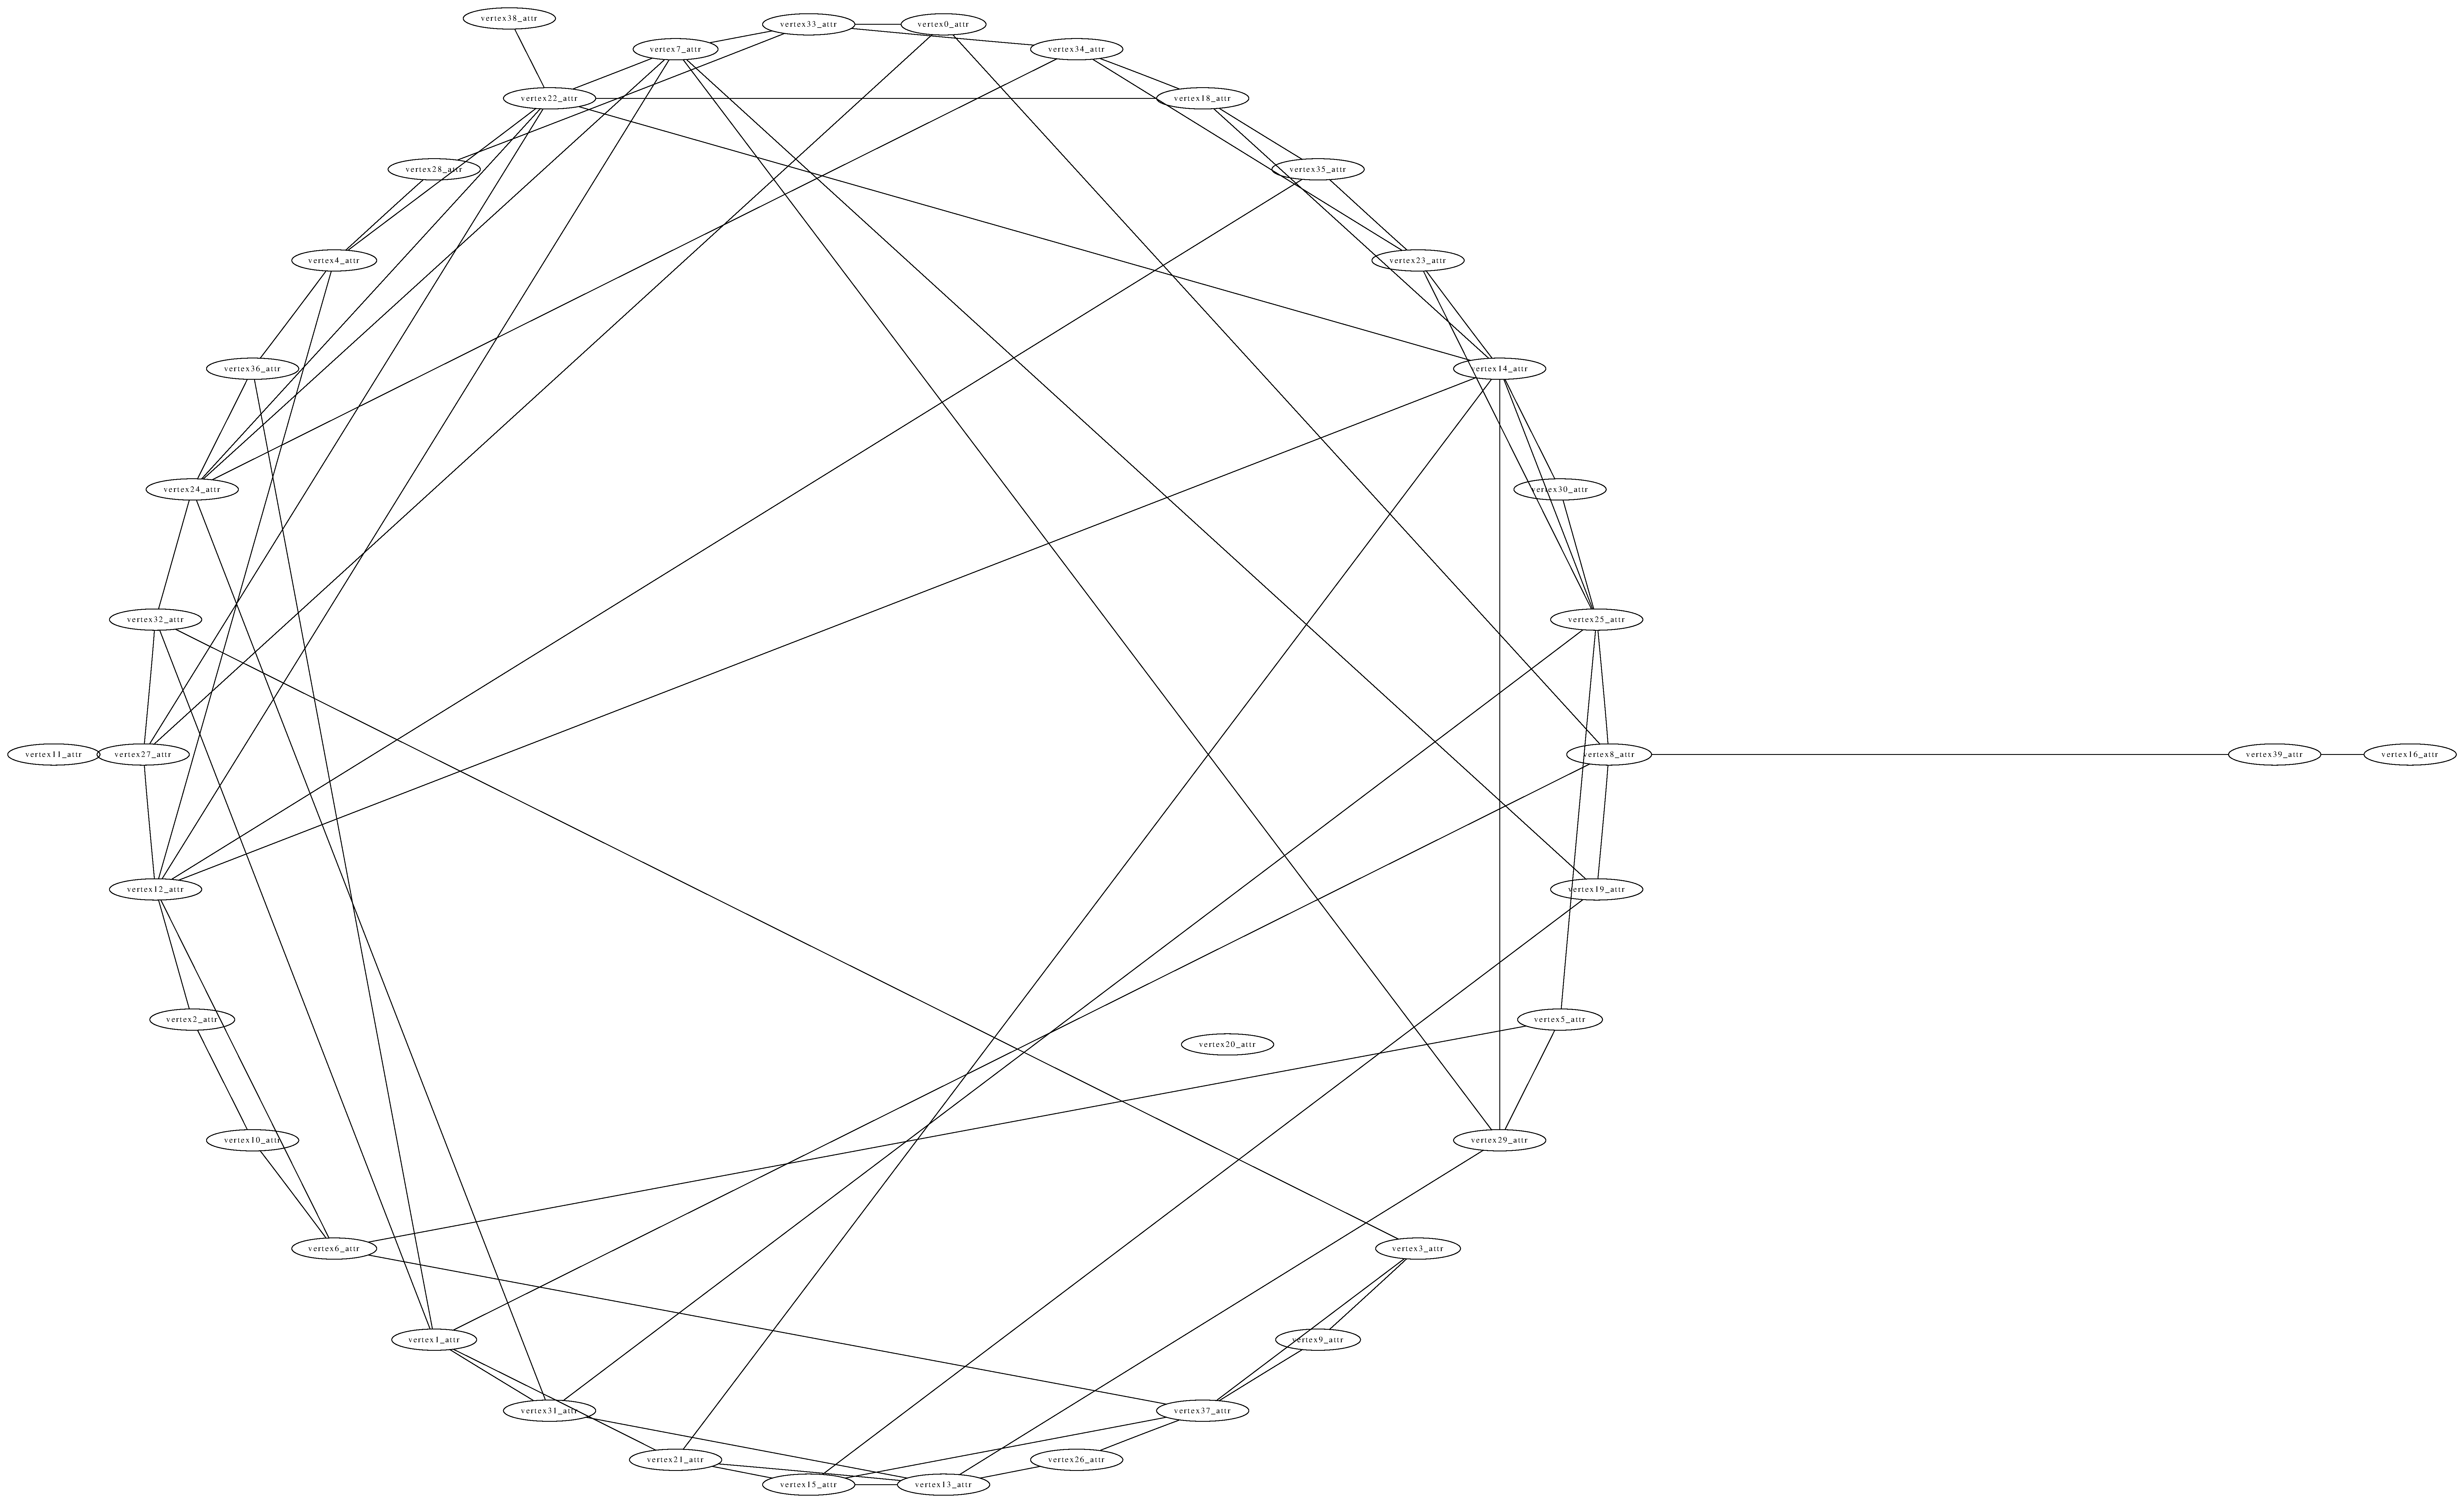
\includegraphics[width=\textwidth]{images/experiments/data/artificial/size/40-80}}
	\subfigure[\dataset{70-245}]{
\includegraphics[width=\textwidth]{images/experiments/data/artificial/size/70-245-fixed}}
\end{figure}

To interpret Tables \ref{table-experiments-data-artificial} and \ref{table-experiments-data-artificial-size}: we get 3 sets of different sizes and densities in the first one, which should work very nice with our heuristics. The $|V|$ and $|E|$ numbers are orders of magnitude higher than with any realistic (or converted) data set we are using, and this will put real stress on the heuristics, as we shall see in the next section.

In the second table we aimed for the $\frac{|E|}{E_{max}}$ density of $0.1 = 10\%$, and we can see that this was quite nicely achieved. There is an interesting observation to be made here: the optimum is steadily decreasing with the increasing overall graph size. This intuitively suggests that the maximal quality theoretically achievable has to do with the $\frac{|E|}{|V|}$ density, not with the one we fixed. Exploration of this phenomenon is among the possibilities of future work of this thesis.

\section{Experimental Setup}

As was mentioned before, we will be using an extension to the jInfer framework called \jmodule{IDSetSearch}. Please see appendices \ref{appendix-jInfer} and \ref{appendix-iss} for more detailed information on these two pieces of software.\\

We now have to define a few notions before moving forward to the description of our experiments.

\begin{define}[Experiment parameters]
	\label{define-experiment-params}
	\textit{Experiment parameters} are the following.
	\begin{itemize}
		\item All the parameters in all the heuristics.
		\item The specific way in which the heuristics are chained.
		\item Parameters $\alpha$ and $\beta$ in the weight (quality) measurement.
		\item Initial pool size.
		\item The termination criteria.
		\item The input XML file.
		\item Known optimum for this file and $\alpha$, $\beta$.
	\end{itemize}
\end{define}

\begin{define}[Experiment(al) configuration]
	\label{define-experiment-config}
	An \textit{experiment instance}, or \textit{configuration}, is one specific setting of all (experiment) parameters.
\end{define}

\begin{define}[Experiment(al) set]
	\label{define-experiment-set}
	One or more experiment configurations, regardless whether their parameters differ, constitute an \textit{experimental set}.
\end{define}

\subsection{Grammar and Model Creation}

TODO link BasicIGG to see how we get IG

TODO describe how we get the model

\subsection{Hardware and Software}

We will be using two different machines to run the experiments. Every experimental result will have explicitly stated the machine it was performed on, and we shall make sure to run different experiments that can benefit from side-by-side comparison on the same machine.

\subsubsection{Quad Core Machine}

\begin{verbatim}
Intel Core 2 Quad processor @ 2.83 GHz
8 GB DDR2 RAM
Windows 7 SP1 64bit
TODO
TODO
GLPK version TODO
\end{verbatim}

\subsubsection{Dual Core Machine}

\begin{verbatim}
Intel Core 2 Duo processor @ 2.33 GHz
4 GB DDR2 RAM
Windows 7 SP1 64bit
Java SE Runtime Environment (build 1.6.0_26-b03)
Java HotSpot 32-Bit Client VM (build 20.1-b02)
GLPK version 4.45 (Cygwin)
GLPK version 4.34 (native)
\end{verbatim}

\subsection{Methodology}

It is impossible to completely shield an experiment from the influence of the environment, but we should try our best. First of all, NetBeans running the experiments is the only relevant program running in the system at that time, as far as this is possible. Unfortunately, the NetBeans itself is quite a large environment with a life on its own, and we would most certainly get more reliable results, if we could run our experiments outside it. This improvement is left for the future work.

Also, every experimental configuration is run 20 times in hope that the effects of any events adversely affecting our results (e.g. OS deciding to run some house cleaning) will be averaged out. Whenever possible, we will always be using boxplots instead of a simple average (or average and variance) to present results of these multiple runs. % TODO discuss caches and the order in which we run the experiments in one set?

\subsection{Measuring the time}

TODO

\subsection{Obtaining the results}

Every run of an experiment produces a trace such as the one presented and commented on in Appendix \ref{appendix-trace}. We can get all the information relevant to that experiment run from this trace alone. An experimental set will produce a number of these traces and store them in plain text files in a folder. Parsing these files to aggregate and collate them might be a tedious task even using tools like \texttt{sed} and \texttt{grep}, so some of the experiment sets directly output tabular data in format recognized by GnuPlot, which we use to plot charts found in this work.

\section{Experimental Results}

\subsection{Grammar and model generation}

%         NB class GrammarModelTiming

The first experiment set will try to establish how long it takes to extract the IG % TODO IG -> nomenclature
from the input XML file and how long does it take to create the AM model from this IG. For now, we will not be running or measuring any heuristics.

\begin{center}
\bigskip
\begin{tabular}{| l | l |}
  \hline
  \hline
  Machine           & TODO \\
  Input data        & all official and sized test data sets \\
  Iterations        & 20 \\
  Pool size         & not applicable \\
  $\alpha$, $\beta$ & not applicable \\
  \hline
\end{tabular}
\bigskip
\end{center}

The experimental set will contain $20 * (11 + 11) = 440$ configurations: 20 iterations for 11 test data sets plus 11 sized test data sets. There will be no CHs or IHs. We will be gathering the timing data for IG extraction and model generation in GnuPlot format.

\placeholder

TODO graph + interpretation

\subsubsection{GLPK interface timing}

%         NB class GlpkInterfaceTiming

A related problem is how long it takes to create input for GLPK and then parse its results. We will use the same test data sets as in the previous case, but now we will gather times needed to communicate with GLPK.

\placeholder

TODO graph + interpretation

\subsection{GLPK: native vs. Cygwin}

%         NB class TimeQuality
%         NB class TimeTillOptimum

In this experiment we will try to remove one of the variables out of the equation: that is the effect of different versions of GLPK on the overall results. The rationale is this: on Windows systems, the two most accessible ways to install GLPK are via a binary distribution TODO link, or via Cygwin as one of its packages.

If we find out which of these Cygwin version is better, we will be using it exclusively without very much fear that this could affect any other aspect of our experiments. We might also find that there is no relevant difference, which would be good, too.

Apart from comparing different versions, we shall see how the pure GLPK approach behaves. The first part of this experiment will be limiting the run time, thus making it an instance of Truncated branch \& bound. In this case we will see the dependency between the run time and the quality achieved in it. In the second time we will let GLPK run until optimum is found. We shall see the dependency between input size and run time needed to achieve the optimum.

\begin{center}
\bigskip
\begin{tabular}{| l | l |}
  \hline
  \hline
  Machine           & Dual Core \\
  Input data        & \texttt{100-500} \\
  Iterations        & 20 \\
  Pool size         & 1 \\
  $\alpha$, $\beta$ & $1$, $1$ \\
  \hline
\end{tabular}
\bigskip
\end{center}

Our experimental set will contain 500 experimental configurations for each of these two GLPK version. Every configuration will use \heu{Glpk} CH set to a time limit from 1 to 49 seconds with increments of 2, meaning 25 settings * 20 iterations = 500 configurations in total (see Listing \ref{listing-experiment-glpk-native-vs-cygwin-1}). There will be no improvement heuristic. The only data we gather in the GnuPlot file are the final qualities (weights).

\begin{algorithm}
\caption{GLPK: native vs. Cygwin set generation 1}
\label{listing-experiment-glpk-native-vs-cygwin-1}
\begin{algorithmic}
\ENSURE experimental set $ES$
\STATE $ES \gets \emptyset$
\FOR{$i = 1 \to 20$}
	\FOR{$time = 1 \to 49$ step $2$}
    \STATE $ES \gets ES \cup {CH = \heu{Glpk}(limit = time), IH = \emptyset}$
  \ENDFOR
\ENDFOR
\RETURN $ES$
\end{algorithmic}
\end{algorithm}

\placeholder

TODO graph + interpretation

\begin{center}
\bigskip
\begin{tabular}{| l | l |}
  \hline
  \hline
  Machine           & Dual Core \\
  Input data        & all sized test data sets \\
  Iterations        & 20 \\
  Pool size         & 1 \\
  $\alpha$, $\beta$ & $1$, $1$ \\
  \hline
\end{tabular}
\bigskip
\end{center}

Another way to compare the performance of these two GLPK versions is to see how long it takes them to find the optimum for a set of data of increasing size. This experimental set will contain 220 configurations for each version. Every configuration will let \heu{Glpk} CH run for unlimited time, until it finds the optimum. This will be repeated in 20 iterations for each of the 11 files from the sized test data set (see Listing \ref{listing-experiment-glpk-native-vs-cygwin-2}). There will again be no IH, the only data we will collect are the times of the CH run in each case.

\begin{algorithm}
\caption{GLPK: native vs. Cygwin set generation 2}
\label{listing-experiment-glpk-native-vs-cygwin-2}
\begin{algorithmic}
\ENSURE experimental set $ES$
\STATE $ES \gets \emptyset$
\FOR{$i = 1 \to 20$}
	\FOR{$file \in $ sized test data}
    \STATE $ES \gets ES \cup \{file, CH = \heu{Glpk}(no\:limit), IH = \emptyset\}$
  \ENDFOR
\ENDFOR
\RETURN $ES$
\end{algorithmic}
\end{algorithm}

\placeholder

TODO graph + interpretation. Graph should have its Y axis in log, stress this fact in the text too

TODO mention that these times show we cannot rely on GLPK alone! It just takes too long.

\subsection{\heu{Random} vs. \heu{Fuzzy} vs. \heu{FIDAX}}

%         NB class RandomVsFuzzyVsFidaxStart

Our investigation into various CH will start by comparing \heu{FIDAX} from the original article \cite{fidax} to 2 of our trivial randomized hungry heuristics, \heu{Random} and \heu{Fuzzy}.

\begin{center}
\bigskip
\begin{tabular}{| l | l |}
  \hline
  \hline
  Machine           & TODO \\
  Input data set    & all official test data sets \\
  Iterations        & 20 \\
  Pool size         & 10 \\
  $\alpha$, $\beta$ & $1$, $1$ \\
  \hline
\end{tabular}
\bigskip
\end{center}

The experimental set will contain 660 configurations in total: 3 different CHs * 11 official test data sets * 20 iterations. There will be no improvement heuristics. The pool size will be set to 10, even though \heu{FIDAX} cannot not profit from this. Listing for this can be found in \ref{listing-experiment-random-fuzzy-fidax}.

We will be gathering the running time of the CH itself and incumbent qualities (best in the pool) for GnuPlot.

\begin{algorithm}
\caption{Random vs. Fuzzy vs. FIDAX set generation}
\label{listing-experiment-random-fuzzy-fidax}
\begin{algorithmic}
\ENSURE experimental set $ES$
\STATE $ES \gets \emptyset$
\FOR{$i = 1 \to 20$}
	\FOR{$file \in $ official test data}
    \STATE $ES \gets ES \cup \{file, CH = \heu{Random}(pool = 10), IH = \emptyset\} \cup \{file, CH = \heu{Fuzzy}(pool = 10), IH = \emptyset\} \cup \{file, CH = \heu{FIDAX}, IH = \emptyset\}$
  \ENDFOR
\ENDFOR
\RETURN $ES$
\end{algorithmic}
\end{algorithm}

\placeholder

TODO graphs (files with similar behavior together) + interpretation.

\subsubsection{Improving \heu{FIDAX} with \heu{Hungry}}

%         NB class FidaxWithHungry

There is a minor question to be answered easily: is \heu{FIDAX} ``hungry enough"? Could we improve it using \heu{Hungry} as IH? Let us design a short experiment.

\begin{center}
\bigskip
\begin{tabular}{| l | l |}
  \hline
  \hline
  Machine           & Dual Core \\
  Input data set    & all official test data sets \\
  Iterations        & 1 \\
  Pool size         & 1 \\
  $\alpha$, $\beta$ & $1$, $1$ \\
  \hline
\end{tabular}
\bigskip
\end{center}

We won't be needing pool bigger than one, nor more iterations - both \heu{FIDAX} and \heu{Hungry} are deterministic. We will try all official data sets, first with empty IH, second with \heu{Hungry} as IH. We will gather the qualities in each case and see whether there is any improvement.

The experimental results are summarized in the Table \ref{table-experiments-fidax-and-hungry} and are quite surprising. As trivial a heuristic \heu{Hungry} is, it is still able to improve the ID set found by \heu{FIDAX} by as much as almost 50\% (the last row, \dataset{100-1000}).

Table \ref{table-experiments-fidax-and-hungry-idsets} lists the ID attributes found in both cases for this most extreme input, \dataset{100-1000}. Note that the content of each cell means ``attribute \texttt{attr} in element \texttt{vertexXY} should be marked as ID attribute".

\begin{table}
  \caption{Results of adding \heu{Hungry} after \heu{FIDAX}}
  \bigskip
  \label{table-experiments-fidax-and-hungry}
  \centering
  \begin{tabular}{l | l | l}
    Data set & Quality - \heu{FIDAX} & Quality - \heu{FIDAX} + \heu{Hungry} \\
    \hline
    \dataset{OVA1}     & 0.4411764705882353  & 0.4411764705882353   \\
    \dataset{OVA2}     & 0.16346153846153846 & 0.16346153846153846  \\
    \dataset{OVA3}     & 0.25482414123443264 & \textbf{0.2553715615163541}   \\
    \dataset{XMA-c}    & 0.7546666666666666	 & 0.7546666666666666   \\
    \dataset{XMA-p}    & 0.2019306150568969	 & 0.2019306150568969   \\
    \dataset{XMD}      & 0.09786094165493509 & 0.09786094165493509  \\
    \dataset{MSH}      & 0.5416472778036296	 & 0.5416472778036296   \\
    \dataset{NTH}      & 0.05259709474828076 & \textbf{0.057918595422124436} \\
    \dataset{100-100}  & 0.56	               & \textbf{0.6766666666666669}   \\
    \dataset{100-200}  & 0.44200000000000017 & \textbf{0.5980000000000003}   \\
    \dataset{100-1000} & 0.19952380952380955 & \textbf{0.29619047619047617}  \\
  \end{tabular}
\end{table}

% TODO for some reason \texttt{\textbf{vertex5}} looks only like \texttt{vertex5}
\begin{table}
  \caption{ID sets in \heu{FIDAX} versus \heu{FIDAX} + \heu{Hungry}}
  \bigskip
  \label{table-experiments-fidax-and-hungry-idsets}
  \centering
  \begin{tabular}{l | l}
  \heu{FIDAX} & \heu{FIDAX} + \heu{Hungry} \\
  \hline
                    & \texttt{\textbf{vertex5}}  \\
                    & \texttt{\textbf{vertex26}} \\
  \texttt{vertex30} & \texttt{vertex30} \\
  \texttt{vertex31} & \texttt{vertex31} \\
  \texttt{vertex32} & \texttt{vertex32} \\
  \texttt{vertex34} & \texttt{vertex34} \\
  \texttt{vertex35} & \texttt{vertex35} \\
  \texttt{vertex36} & \texttt{vertex36} \\
  \texttt{vertex37} & \texttt{vertex37} \\
  \texttt{vertex39} & \texttt{vertex39} \\
                    & \texttt{\textbf{vertex60}} \\
                    & \texttt{\textbf{vertex69}} \\
                    & \texttt{\textbf{vertex70}} \\
  \texttt{vertex74} & \texttt{vertex74} \\
  \texttt{vertex75} & \texttt{vertex75} \\
  \texttt{vertex80} & \texttt{vertex80} \\
  \end{tabular}
\end{table}

\subsection{Best standalone CH}

%         NB class BestStandaloneCH

TODO compare all CHs - limit GLPK to ~ 1 second
TODO pool size 10 where applicable

TODO chart for each file: CHs on the X axis, quality Y axis, boxplots

\begin{center}
\bigskip
\begin{tabular}{| l | l |}
  \hline
  \hline
  Machine           & TODO \\
  Input data        & all official test data sets \\
  Iterations        & 20 \\
  Pool size         & 10 \\
  $\alpha$, $\beta$ & $1$, $1$ \\
  \hline
\end{tabular}
\bigskip
\end{center}

\placeholder

\placeholder

\placeholder

\subsection{Best IH for the best CH}

TODO with the best construction heuristic, which IH is the best? Note that this needn't be the best combination!

\subsubsection{\heu{Random} as CH}

TODO with the best IH from the previous step, how about using Random as CH?

\subsection{Various $\alpha$, $\beta$}

TODO remind what these parameters mean

\subsubsection{Effects on performance}

TODO

\subsubsection{Effects on the ID set}

TODO

\subsection{Ignoring text data}

TODO can we improve performance on huge data by ignoring textual content? Check for building as well as actual heu times.

\subsection{Chaining the IHs}

TODO finally we got to the most interesting part, unfortunately this is basically guesswork and intuition.

\subsection{Algorithms for various data characteristics}

TODO

\section{The "Best" Algorithm}

TODO we have asked a lot of questions and got the answers, now is the time to summarize, to find some "wisdom".

First of all: if we have the time, it is best to just let the GLPK run.
We will find the optimum in this way.
And for many purposes, this is just fine - we need to infer something about the schema, we do it only once, so it doesn't matter that much how long it takes.

Second: if we don't have enough time, we should do XYZ but it might depend on the characteristics of the data.
For realistic (looks like THIS in graph representation) it is best to do A B C.
Whereas, for artificial data (having IJK as their representation) it is best to just do 1 2 3.
